
% !TEX root = DesignDocument.tex

\chapter{Design  and Implementation}

\section{Systems Goals}
Briefly describe the overall goals this system plans to achieve.
These goals are typically provided by the stakeholders.  This is not
intended to be a detailed requirements listing.  Keep in mind that
this section is still part of the Overview.

\section{System Overview and Description}
Provide a more detailed description of the major system components
without getting too detailed.  This section should contain a
high-level block and/or flow diagram of the system highlighting the
major components.  See Figure~\ref{systemdiagram}.  This is a floating
figure environment.  \LaTeX\ will try to put it close to where it was
typeset but will not allow the figure to be split if moving it can not
happen.  Figures, tables, algorithms and many other floating
environments are automatically numbered and placed in the appropriate
type of table of contents.  You can move these and the numbers will
update correctly.

\begin{figure}[tbh]
\begin{center}
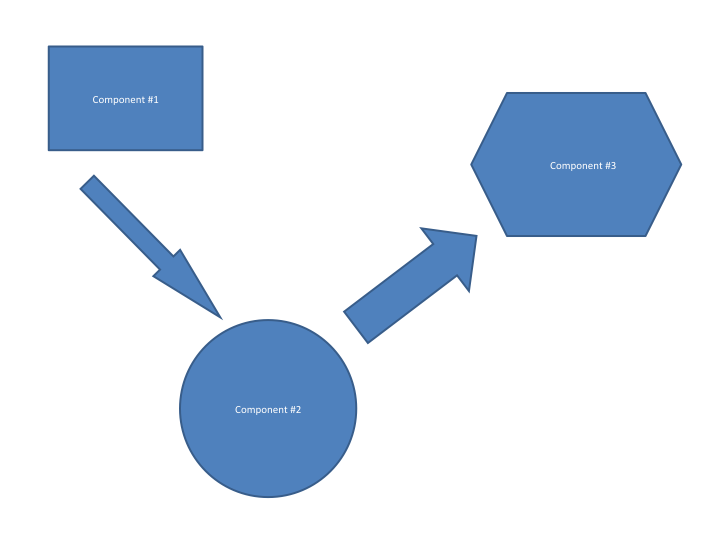
\includegraphics[width=0.75\textwidth]{./diagram}
\end{center}
\caption{A sample figure .... System Diagram \label{systemdiagram}}
\end{figure}

\subsection{Website}
Describe briefly the role this major component plays in this system. 

\subsection{File Conversion}
The file conversion software converts files between common 3D file types.  It is designed to 
be called from the back end of the website.

Table \ref{table:suportedfiletypes} lists the minimum file types supported.  More may be supported, but those listed are the minimum needed to support the majority of common file types.  
Models created in most common Computer Aided Design software can export to some of the input file types.

\begin{table}[!h]
    \centering
    \begin{tabular}{| c | c |}
        \hline
        Input file type & Output file type \\
        \hline
        .fbx & .fbx \\
        .dae & .dae \\
        .blend & .obj \\ 
        .obj & .stl \\
        .stl & .ply \\
        .ply & \\
        \hline
    \end{tabular}
    \caption{Supported File Types}
    \label{table:suportedfiletypes}
\end{table}

\section{Technologies Overview}
This section should contain a list of specific technologies used to
develop the system.  The list should contain the name of the
technology, brief description, link to reference material for further
understanding, and briefly how/where/why it was used in the system.
See Table~\ref{somenumbers}.  This is a floating table environment.
\LaTeX\ will try to put it close to where it was typeset but will not
allow the table to be split.

\begin{table}[tbh]
\caption{A sample Table ... some numbers. \label{somenumbers}}
\begin{center}
\begin{tabular}{|r|l|}
  \hline
  7C0 & hexadecimal \\
  3700 & octal \\ \cline{2-2}
  11111000000 & binary \\
  \hline \hline
  1984 & decimal \\
  \hline
\end{tabular}
\end{center}
\end{table}


 \section{Architecture and System Design}
This is where you will place the overall system design and the architecture.   This section will be very detailed and should be image rich.  There is the old phrase {\it a picture is worth a thousand words}, in this class it could be worth hundreds of points (well if you sum up over the entire team).   One needs to enter the design and why a particular design has been done.   THIS IS THE CORE OF THE COURSE.    
 
 
 {\it It is important for you to say why as much as what.   }
 
   \subsection{Design Selection}
 Failed designs, design ideas, rejected designs here.
 
 \subsection{Data Structures and Algorithms}
 Describe the special data structures and any special algorithms.
 
 \subsection{Data Flow}
 
 \subsection{Communications}
 
 \subsection{Classes}
 
 \subsection{UML}
 
 \subsection{UX}
 
 \subsection{UI}
 
 \subsection{MVVM, etc}

 \section{Website}

 \section{File Conversion}

    \subsection{Overview}
    \paragraph{}
    A major tool in the project is the File Conversion Software.  
    The file conversion software aims to read in many different 3D model file types (.fbx, .obj, .dae, ...) and convert them to another desired 3D file type.  
    A brief listing of suported file types is in table \ref{table:suportedfiletypes}.

    \paragraph{}
    This tool is intended to be used on the back end of the website.  Whenever a user uploads a file, it can be converted to a common file type, using this tool.
    When the user requests a download on an AR device, the type may be different than what is stored.  Therefore, the tool will be used to convert the file before
    it is sent to the user.

    \paragraph{}
    Since this tool is intended to be used on the backend of a website, it is appropriate to use a command line interface.  
    The flags that can be passed to the program are listed below:

    \begin{table}[h]
        \centering
        \begin{tabular}{l  l}
            -i & Input file name (can specify full path), infers the input file type from the name \\
            -o & Name (or full path) to write the converted file, infers the export file type from the name \\
            -odir & The path to the directory, the file name is inferred from the input file name \\
            -t & The file type (.fbx, .obj, .dae, ...) to export to
        \end{tabular}
    \end{table}

    Note the -t flag is only needed when using the -odir flag.  The -odir just specifies which directory to write to, but not the file type.
    Therefore, more information is needed in order to export to a file.  The -o flag will parse the file name and extract the file type from the -i file name.

    An example command to run:

    \begin{center}
        .\textbackslash FileConversion.exe -i C:\textbackslash SomePath\textbackslash someFile.obj -t fbx -odir C:\textbackslash SomeOtherPath\textbackslash
    \end{center}

    This will convert a file named someFile.obj located at C:\textbackslash SomePath\textbackslash  to an FBX file named someFile.fbx located at 
    C:\textbackslash SomeOtherPath\textbackslash

    \subsection{Technologies Used}

    The code for the file conversion toolset is written in C++.  There are two main external libraries used:
    \begin{itemize}
        \item Open Asset Import Library (assimp)
        \begin{itemize}
            \item \url{http://assimp.org/main_downloads.html}
        \end{itemize}

        \item FBX SDK
        \begin{itemize}
            \item \url{http://usa.autodesk.com/adsk/servlet/pc/item?siteID=123112&id=26416244}
        \end{itemize}
    \end{itemize}

    Multiple librarires are needed to support the file types that are necessary for common AR rendering.  In the Microsoft Hololens, the default
    3D viewer supports FBX files very easily.  Therefore, it was decided that the conversion software needed to export to FBX.  The best tool to do 
    so is the FBX SDK, since FBX is a propriatary file format from Autodesk.  However, the FBX SDK has a very limited range of file types it will read and write.
    Therefore, the Open Asset Import Library is used to better support a wide array of file types.  So in using assimp and the FBX SDK together,
    the converison software can support a wide range of both import and export file types.

    \subsection{Data Flow}
        There are four main paths data can flow.
        \begin{itemize}
            \item assimp
            \begin{itemize}
                \item import and export all with the assimp library
            \end{itemize}
            
            \item FBX SDK
            \begin{itemize}
                \item import and export all with the FBX SDK library
            \end{itemize}

            \item assimp $\rightarrow$ FBX SDK
            \begin{itemize}
                \item import with assimp, export to temporary file type
                \item import temporary file with FBX SDK, export to final file 
            \end{itemize}

            \item FBX SDK $\rightarrow$ assimp
            \begin{itemize}
                \item import with FBX SDK, export to temporary file type
                \item import temporary file with assimp, export to final file 
            \end{itemize}
        \end{itemize}
        
        This outlines that the program tries to use a single library to convert the file before using multiple.  If a single library is unable to 
        read and write the needed formats, it tries to import with one, export to a temporary format, and export with the other.  An example of 
        using a single library is if a user wants to read a .obj and write to a .fbx.  The FBX SDK can handle reading and writing those particular file
        types, so it will be used ot do the conversion.  An example of needing to use both libraries is if a user wants to convert a .ply to a .fbx.
        Assimp can read .ply files, but cannot write to .fbx.  The FBX SDK can write to .fbx files but not read .ply.  Therefore, assimp is used to 
        read the .ply, write to a .dae (common file type).  The FBX SDK then reads the .dae and writes to a .fbx.

    \subsection{Design Details}

    \subsubsection{Overview}

    The file converison software is written in C++.  The structure of the program is object oriented, where classes are defined where the functionality needed
    in the program is defined.  Instances of the classes will be created when needed.  
    The high level view of the program is:
    \begin{enumerate}
        \item Parse command line arguments
        \item Convert the file
        \item Print error messages if errors occured
    \end{enumerate}

    The parsing the command line arguments section may fail if the user does not supply the correct arguments.  A flag is set after parsing to indicate
    whether the correct arguments were supplied.  If an error occurrs during file conversion, the error will be denoted by an integer error code.  
    During file conversion, if a single library could not convert it on its own, an extra file will be created as an intermediate file.

    \subsubsection{Code Structure}
    The file conversion software is broken into two main sections: parameter parsing and file conversion.

    \paragraph{Parameter Parsing}
    \hfill \break
    The parameter parsing code is in a class called ParseParameters.  ParseParameters has a constructor that takes the number of command line arguments, 
    and the command line arguments.  It will parse the values needed out into member variables that are public.  It will ignore invalid arguments,
    and print a usage statement if the correct arguments are not supplied.  When printing the useage statement, cout is used to write to standard out.

    After processing the command line arguments, the member variables in the class will be set with the appropriate information.  The member variables are:

    \begin{tabular}{l l}
        \centering
        success & bool \\
        & True if the needed information is set, false otherwise \\

        inputFile & string \\
        & The name/path of the file to convert \\

        outputFile & string \\
        & The name/path of the file to export to \\

        fileExtention & string \\
        & The file extention of the output file
    \end{tabular}

    If the success variable is false, the other member variables possibly have bad data that should not be used.

    \paragraph{File Conversion}
    \hfill \break
    The file conversion portion of the progarm is the meat of the functionality.  It takes an input file, and tries to convert it to the file type requested.
    This seciton implements the two libraries.  Each library is implemented in a class inherited from an abstract AbstractConverter converter class.  The two 
    library implementation classes are called AssimpConverter and FBXConverter.  A class named FileConverter contains the logic on determining which 
    library/libraries to use when converting the file.

    \subparagraph{AbstractConverter}
    \hfill \break
    The AbstractConverter is an abstract class that acts like an interface for the child classes.  The abstract methods are:
    \begin{itemize}
        \item SupportsInputFileType
        \begin{itemize}
            \item Return true if the converter can read in a file with a given file type
        \end{itemize}

        \item SupportsOutputFileType
        \begin{itemize}
            \item Return true if the converter can write to a file with a given type
        \end{itemize}

        \item ConvertFile
        \begin{itemize}
            \item Performs the file conversion
        \end{itemize}
    \end{itemize}

    An emum is defined, called Result, that provides a more self documenting way to return information from functions.  Values less than zero are errors, while
    value greater than zero are successes.  The levels of the enum are:
    
    \begin{tabular}{l l}
        \centering
        Failed &\\
        IOError &\\
        SceneNotLoaded &\\
        NotInitialized &\\
        FileTypeNotSupported &\\
        Success &
    \end{tabular}

    \subparagraph{AssimpConverter}
    \hfill \break
    The AssimpConverter inherits from the AbstractConverter and uses the Open Asset Import Library for file conversion.  
    The file type supported methods are implementd by adding the supported file types to a set, and checking whether the questionable type is in the set.
    The list of file types supported is taken from the Open Asset Import Library website's list of supported input file types.  
    The output file types list comes from the same location.
    When converting a file, optimizations may be performed on the file to remove unnecessary/duplicate information.  For example, when importing a file, 
    repeatedverticies in the meshes will be condensed into one, to help reduce the size of the file.

    \subparagraph{FBXConverter}
    \hfill \break
    The FBXConverter inherits the AbstractConverter and uses the FBX SDK to import and export files.
    THe file type input and output lists are derived from the FBX SDK website.

    \subparagraph{FileConverter}
    \hfill \break
    The FileConverter looks at the input and output file types, and determines which library/libraries needed to convert the file.
    It tries see if a single library can do the conversion.  If not, then both libraries are used by exporting from one into a 
    temporary file (.dae) and converting that to the final file type. After comparing the read/write lists between the libraries,
    the DAE file type was common between the two, and included features that other file types did not.  Therefore, it was chosen
    to have DAE as the common intermediate file type.

 \begin{comment}
    \section{Major Component \#1 }

    {\bf If the following makes sense, use this outline, if not then modify the outline}


    This section is used to describe the design details for each of the major components 
    in the system.    Note that this chapter is critical for all tracks.  Research tracks would do experimental design here where other tracks would include the engineering design aspects.    This section is not brief and requires the necessary detail that 
    can be used by the reader to truly understand the architecture and implementation 
    details without having to dig into the code.    Sample algorithm:  Algorithm~\ref{alg1}.  This algorithm environment is automatically placed - meaning it floats.   You don't have to worry about placement or numbering.  

    \begin{algorithm} [tbh]                     % enter the algorithm environment
    \caption{Calculate $y = x^n$}          % give the algorithm a caption
    \label{alg1}                           % and a label for \ref{} commands later in the document
    \begin{algorithmic}                    % enter the algorithmic environment
        \REQUIRE $n \geq 0 \vee x \neq 0$
        \ENSURE $y = x^n$
        \STATE $y \Leftarrow 1$
        \IF{$n < 0$}
            \STATE $X \Leftarrow 1 / x$
            \STATE $N \Leftarrow -n$
        \ELSE
            \STATE $X \Leftarrow x$
            \STATE $N \Leftarrow n$
        \ENDIF
        \WHILE{$N \neq 0$}
            \IF{$N$ is even}
                \STATE $X \Leftarrow X \times X$
                \STATE $N \Leftarrow N / 2$
            \ELSE[$N$ is odd]
                \STATE $y \Leftarrow y \times X$
                \STATE $N \Leftarrow N - 1$
            \ENDIF
        \ENDWHILE
    \end{algorithmic}
    \end{algorithm}
    Citations look like~\cite{Choset:2005:PRM, arkin2009governing, lavalle2006}  and~\cite{wiki:asimo,lumelsky:1987, nolfi2000evolutionary}.  These are done automatically.  Just fill in the database {\tt designrefs.bib} using the same field structure as the other entries.  Then pdflatex the document, bibtex the document and pdflatex twice again.  The first pdflatex creates requests for bibliography entries.
    The bibtex extracts and formats the requested entries.  The next pdflatex puts them in order and assigns labels.  The final pdflatex replaces references in the text with the assigned labels.
    The bibliography is automatically constructed.  
    


    \subsection{Technologies  Used}
    This section provides a list of technologies used for this component.  The details 
    for the technologies have already been provided in the Overview section. 

    \subsection{Component  Overview}
    This section can take the form of a list of features. 

    \subsection{Phase Overview}
    This is an extension of the Phase Overview above, but specific to this component. 
    It is meant to be basically a brief list with space for marking the phase status. 

    \subsection{ Architecture  Diagram}
    It is important to build and maintain an architecture diagram.  However, it may 
    be that a component is best described visually with a data flow diagram. 


    \subsection{Data Flow Diagram}
    It is important to build and maintain a data flow diagram.  However, it may be 
    that a component is best described visually with an architecture diagram. 


    \subsection{Design Details}
    This is where the details are presented and may contain subsections.   Here is an example code listing:
    \begin{lstlisting}
    #include <stdio.h>
    #define N 10
    /* Block
    * comment */
    
    int main()
    {
        int i;
    
        // Line comment.
        puts("Hello world!");
    
        for (i = 0; i < N; i++)
        {
            puts("LaTeX is also great for programmers!");
        }
    
        return 0;
    }
    \end{lstlisting}
    This code listing is not floating or automatically numbered.  If you want auto-numbering, but it in the algorithm environment (not algorithmic however) shown above.

\end{comment}
